\section{Theoretical Justification of Robustness}
\label{sec:bl_justification}

In Section~\ref{ssec:bayesianLearning}, we discussed how a Bayesian approach to
regression achieves bias-variance trade-off and combats the risk of overfitting. 
%
We translate the same idea to the data-driven control design problem.
%
For instance, the \textsc{NeuralPbc} framework discussed in
Section~\ref{ssec:pbc} assumes a nominal system model given by $f(x, u)$.
%
The parameters of the desired Hamiltonian are updated from a finite dataset
generated from this model.
%
A robust controller would not overfit to a point-estimate with the assumption
that the finite trajectory observations represent the real system. 
%
System parameter and measurement uncertainties in the real system can generate
vastly different trajectories, which the deterministic (point-estimate)
controller may find foreign.
%
We propose a Bayesian learning framework where the controllers are given by
stochastic functions.
%
In this framework, we achieve the performance objective with wide range of
control inputs sampled from the stochastic control, which can be viewed as
training \textit{an ensemble of controllers}.
%
\textit{This provides a conservative control policy that is robust to uncertainties}.


The variance in the stochastic control is the most beneficial when there is an
unknown discrepancy between the nominal model and the real system.
%
In this section, we show the relationship between the model uncertainties and
the variance of the stochastic control.
%
We also demonstrate the significant effects of these model discrepancies on the
performance objective and the improved robustness properties of Bayesian
learning over point-estimates of a policy. This theoretical justification is
given by a toy example, where closed-form calculation of the point-estimates and
posterior distributions for the optimal controller is provided.

\subsection{Optimal Control under Parameter Uncertainty}
%
Let us consider the first-order scalar control system, whose system parameter
$p_s$ is uncertain: 
%
\begin{equation} \begin{cases} \dot{x} = p_sx + u, \; x(0) =
  x_0, \\ u(x) = \theta x.  \end{cases} \label{eq:first-order} \end{equation}
%
We assume that $p_s \sim \mc{N}\left(\hat{p}_s, \sigma_{p}\right)$ where
$\hat{p}_s$ designates our best prior point estimate of the system parameter $p_s$
and $\sigma_{p} > 0$ quantifies the uncertainty in the knowledge of the system
parameter. The controller is set to be linear in the state $x \in \mathbb{R}$
with its only parameter $\theta \in \mathbb{R}$ to be determined through
optimization. Without loss of generality, we will take the initial condition
$x_0 = 1$. The performance index to be optimized for determining the best
control parameter $\theta$ is
%
\begin{equation} \mc{J} = \int_0^T \left(\frac{1}{2}cx^2 + \frac{1}{2}ru^2 \right) dt,
\label{eq:perfind} \end{equation}
%
where $T$ is the control horizon and $c \geq 0$ and $r > 0$ are design
parameters. We solve the control system~\eqref{eq:first-order} to find $x(t) =
e^{(p_s+\theta)t}$ and plug this into the performance index~\eqref{eq:perfind}
along with the form selected for the controller. Performing the integration over
time and letting $T \to \infty$, assuming that $p_s+\theta < 0$ then yields the
infinite-horizon optimal cost functional
% %
% \begin{equation*} \mc{J} = -\frac{1}{4}\frac{q+r\theta^2}{(p+\theta)}\left( 1 - 
% e^{2T(p+\theta)} \right).  \end{equation*}
% %
% Assuming that $p+\theta < 0$, we let $T \to \infty$ to obtain the infinite-time
% optimal cost functional
% %
\begin{equation} \mc{J}_\infty = -\frac{1}{4}\frac{c+r\theta^2}{p_s+\theta}.
\label{eq:inf-time-integrated-cost} \end{equation}
%
The optimal control parameter $\theta$ may be found as the appropriate root of
$\nabla_\theta \mc{J}_\infty$. 
%
\begin{align} 
    \begin{split} 
        \nabla_\theta \mc{J}_\infty &= -\frac{r}{4}\frac{(p_s+\theta)^2 - \left(p^2
        + \nicefrac{c}{r}\right)}{(p_s+\theta)^2} = 0, \\ 
        \therefore \theta^\star &= g(p_s) :=-p_s - \sqrt{p_s^2 + \nicefrac{c}{r}}, \\
        &\hspace{2mm} g^{-1}(\theta) = \frac{c}{2r\theta} - \frac{\theta}{2}.
    \end{split} 
    \label{eq:optimal_theta} 
\end{align}
%
The fact that $p_s \sim \mc{N}(\hat{p}_s, \sigma_p^2)$ implies that the optimal
control parameter has the probability density function
%
\begin{align*} 
    f_{\theta^\star}(\theta^\star) &= f_p\left(g^{-1}(\theta^\star)\right)
        \abs{\frac{d}{d\theta}g^{-1}(\theta^\star)}, \\ 
        &= \frac{1}{\sigma_p
        \sqrt{2\pi}}\left(\frac{1}{2}\left(1+\frac{c}{r{\theta^\star}^2}\right)\right)
        \exp{\left\{-\frac{1}{2\sigma_p^2}\left(
        \frac{c}{2r\theta^\star} - \frac{\theta^\star}{2} - \hat{p}_s
        \right)^2\right\}}, 
\end{align*}
%
where $f_p$ is the Gaussian probability density function with mean $\hat{p}_s$ and
variance $\sigma_p^2$. 

We can further eliminate the control parameter from the
expression for the optimal cost function $\mc{J}_\infty$ by
substituting for $\theta$ from
equation~\eqref{eq:optimal_theta}, yielding 
%
\begin{align*}
\mc{J}^\star = &h(p_s) := \frac{r}{2}\left( p_s +
\sqrt{p_s^2 + \nicefrac{c}{r}} \right), \\
&h^{-1}(\mc{J}^\star) = \frac{\mc{J}^\star}{r} -
\frac{c}{4\mc{J}^\star}.
\end{align*}
%
Hence, the distribution of the optimal cost conditioned on the system parameter
$p_s$ is 
%
\begin{align*} 
    f_{\mc{J}^\star}(\mc{J}^\star) &=f_p\left(h^{-1}(\mc{J}^\star)\right)
        \abs{\frac{d}{d\theta}h^{-1}(\mc{J}^\star)}, \\
        &= \frac{1}{\sigma_p
        \sqrt{2\pi}}\left(\frac{1}{r} + \frac{c}{4{\mc{J}^\star}^2}\right)
        \exp{\left\{ -\frac{1}{2\sigma_p^2} \left(
        \frac{\mc{J}^\star}{r} - \frac{c}{4\mc{J}^\star} -
        \hat{p}_s\right)^2\right\}}.
\end{align*}
%
Notice that the distribution of both the optimal control parameter and the
optimal cost are elements of the exponential family that are not Gaussian. 

\begin{figure}[tb]
  \centering
  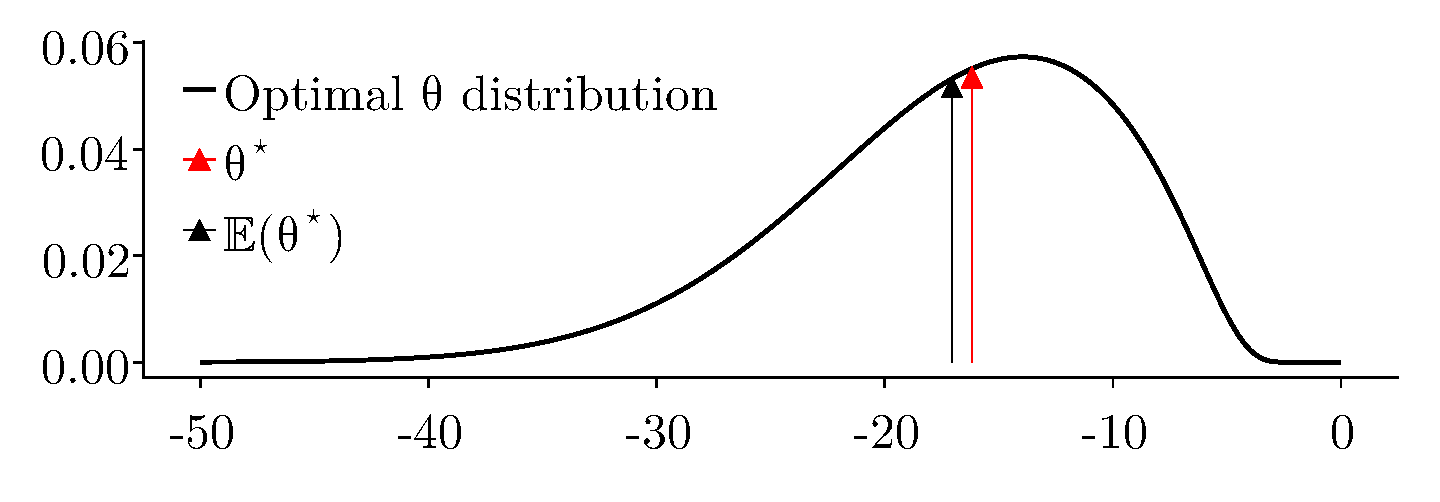
\includegraphics[width=0.7\linewidth]{./figures/optimal-dist.eps}
  \caption{The optimal control parameter distribution given that the system
  parameter $p_s$ is normally distributed with mean $\hat{p}_s = 5$ and $\sigma_p
  = 5$. The red and black arrows respectively indicate the optimal control
  parameter without considering the randomness of $p_s$, and the expected value
  of the optimal control parameter distribution}
  \label{fig:optimal_dist}
\end{figure}


There are several advantages of employing Bayesian learning to find the optimal
control parameter $\theta$ as the toy example in this subsection supports. 
%
In order to derive some quantitative results, let us assign some numerical
values to the parameters that define the optimal cost function $(c,r) = (100, 1)$, our best
guess $\hat{p}_s = 5$ of the system parameter $p_s$ and its standard deviation $\sigma_p = 5$.


The optimal control parameter and cost derived for this system whose model is
assumed to be known perfectly are given by $\hat{\theta}^\star = -16.180$ with
the corresponding estimated cost $\hat{\mc{J}}^\star = 8.090$.
%
This deterministic performance estimate turns out to be \textit{overconfident} when
uncertainties in the system parameter are present. 
%
For example, if the prior knowledge on the distribution of the system parameter
$p_s$ is utilized, the expected value of the controller parameter is found as
$\mathbb{E}[\theta^\star] = -17.046$ and the corresponding expected cost is
$\mathbb{E}[\mc{J}] = 8.523$. 
%
The controller from the deterministic training/optimization is not only
overconfident about its performance; but also is less robust against modeling
errors, as the Bayesian learning yields a closed-loop stable system for a wider
range of values of $p_s$.

Finally, Figure~\ref{fig:optimal_dist} shows the optimal control parameter
distribution given that the system parameter $p_s$ is normally distributed with
mean $\hat{p}_s = 5$, standard deviation $\sigma_p = 5$.
%
This figure also shows the mean values of the optimal control distribution with
the black arrow and the optimal control parameter a deterministic approach would
yield in red. 
%
We notice that the Bayesian learning that yields the optimal control parameter
distribution is more concerned about system stability due to the uncertainty in
the parameter $p_s$, a feat that the deterministic training may not reason about.

\subsection{Optimal Control under Parameter Uncertainty and Measurement
Noise}

Consider the scenario in which the system~\eqref{eq:first-order} is also subject
to measurement errors; that is, our measurement model for the state $x$ is
probabilistic and is distributed according to the Gaussian $\mc{N}(x,
\sigma)$. Since the controller uses this measurement to determine its action,
the closed-loop system has to be modelled as a stochastic differential equation
(SDE), given by
%
\begin{equation} 
  \begin{cases} 
    \dd x(t) = (p_s+\theta)x(t) \; \dd t + \theta\sigma \; \dd W_t, \\ x(0) = 1,
  \end{cases} 
  \label{eq:first-order-SDE}
\end{equation}
%
where $W$ denotes the Wiener process~\cite{evans2012introduction}. The initial
state is assumed deterministic and is set to unity for simplicity.  
% The general case where the initial state is arbitrary and
% stochastic follows exactly the same lines of development.
% 
The unique solution to this SDE is given by
%
\begin{equation}
    x(t) = e^{(p_s+\theta)t} + \theta\sigma \int_0^t e^{(p_s+\theta)(t-s)}dW_s.
    \label{eq:sol-sde}
\end{equation}
%
\vspace{-4mm}
\begin{lem}\label{lem:1}
    The conditional expectation $\mathbb{E}\left[\mc{J}\mid p_s\right]$ of the
    performance index~\eqref{eq:perfind} given the system parameter $p_s$ is 
    \begin{align*} 
      \mathbb{E}\left[\mc{J} \mid p_s\right] &=-\frac{1}{4}\frac{c+r\theta^2}{p_s+\theta}
       \left[ \theta^2 \sigma^2 T + \left(1 - e^{2T(p_s+\theta)}\right) \left(1 +
      \frac{1}{2}\frac{\theta^2\sigma^2}{p_s+\theta}\right)\right].  
    \end{align*} 
\end{lem}
%

\begin{proof}
    The proof may be found in the appendix.
\end{proof}
%

%
It is easily shown that this quantity is positive for all $T>0$. Furthermore, it
blows up as the horizon $T$ is extended to infinity. This is not surprising
since a nonzero measurement noise causes the state to oscillate around the
origin, rather than asymptotically converging to it, incurring nonzero cost
all the while.

% As a concrete example, take the values of $q$, $r$ and $p=\hat{p}$ as in
% Table~\ref{tab:case-study} and further let $T=1$ and $\sigma = 0.2$. In this
% case, the deterministic optimal for the controller parameter is
% $\theta_d^\star = -10.916$. Selecting this controller parameter incurs an
% expected cost $\mathbb{E}_W\left[\mc{J}(\theta_d^\star) \mid p \right] =
% 31.473$. On the other hand, the actual (stochastic) optimal of the controller
% parameter may be found by minimizing $\mathbb{E}_W\left[\mc{J} \mid p \right]$
% numerically and it yields $\theta_s^\star = -7.331$ with an expected cost
% $\mathbb{E}_W\left[\mc{J}(\theta_s^\star) \mid p \right] = 21.399$, which is
% smaller than the one provided by the deterministic optimal. 

We have kept the system parameter $p_s$ constant in this analysis so far.
Uncertainty over this variable can be incorporated by taking a further
expectation \[ \mathbb{E}[\mc{J}] := \mathbb{E}_{p_s}\left[\mathbb{E}_W\left[\mc{J}
\mid p_s \right]\right], \] of $\mathbb{E}_W\left[\mc{J} \mid p_s \right]$ over $p_s$,
which must be accomplished numerically as it does not admit a closed-form
expression.  

We can then minimize $\mathbb{E}[\mc{J}]$ over the control parameter in order to
study the effects of both kinds of uncertainties on the optimal controller.
%
Such a study is provided in Figures~\ref{fig:iwp-projections}
and~\ref{fig:iwp-loss}, where we have plotted the optimal control parameter
$\theta^\star$ and the minimal expected cost $\mathbb{E}[\mc{J}]$ as a function
of the standard deviations of the measurement noise $\sigma$ and the system
parameter $\sigma_p$. The constants we used to generate the data are given by
$c=r=1$ and $T=\hat{p}_s=3$. Our first observation is that the magnitude of the
optimal control parameter is an increasing function of system parameter
uncertainty and a decreasing function of measurement uncertainty. Our second
observation is that if the measurement noise is small, then the optimal control
parameter is insensitive to system parameter uncertainty as long as this
uncertainty is small. The optimal cost shares this insensitivity for an even
wider range of values of $\sigma_p$. In a similar vein, if the uncertainty in
the system parameter is large, then the optimal control parameter is insensitive
to the magnitude of the measurement noise. However, the optimal cost is still
sensitive to this quantity.

\begin{figure}[tb]
  \centering
    \begin{minipage}{.48\textwidth}
        \centering
        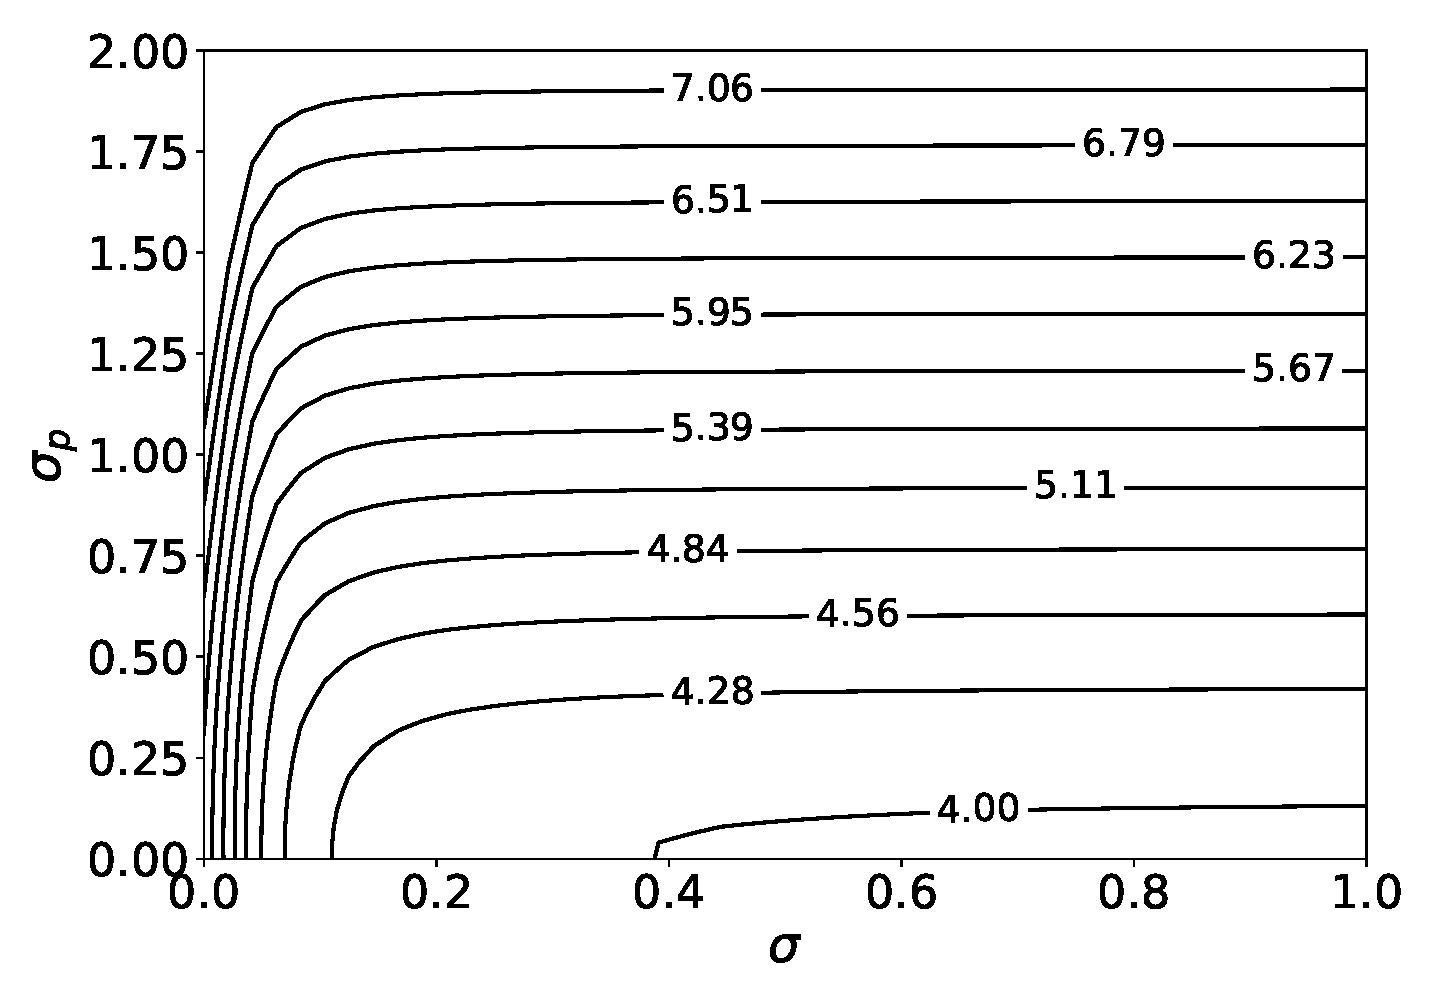
\includegraphics[width=\linewidth]{./figures/optimal_ctrl.eps}
        \caption{The optimal controller parameter magnitude $\abs{\theta^\star}$}
        \label{fig:iwp-projections}
    \end{minipage}%
    \hfill
    \begin{minipage}{0.46\textwidth}
        \centering
        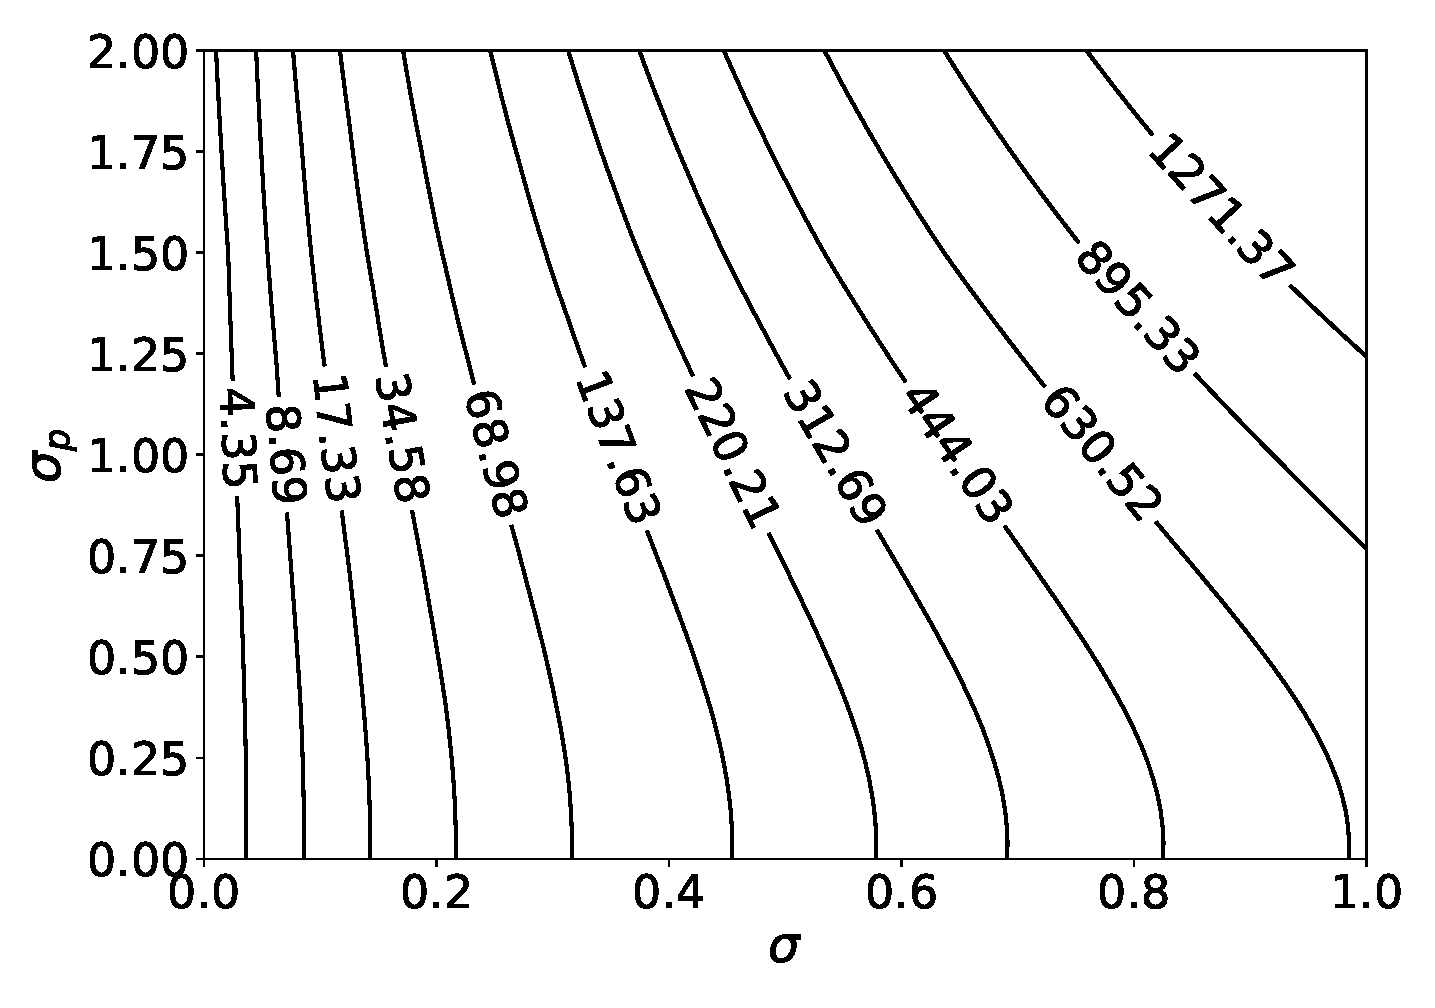
\includegraphics[width=\linewidth]{./figures/optimal_cost.eps}
        \caption{The minimal expected cost $\mathbb{E}[\mc{J}]$}
        \label{fig:iwp-loss}
    \end{minipage}
  % \caption{As a function of the standard deviations of the measurement noise,
  %   $\sigma$, and the system parameter, $\sigma_p$ (a) the magnitude of the optimal
  %   controller parameter $\abs{\theta^\star}$ and (b) the minimal expected cost 
  %   $\mathbb{E}\mc{J}$.}
  %
  \label{fig:optimal-ctrl-cost}
\end{figure}

% \begin{figure}[]
%     \centering
%     %
%     \setkeys{Gin}{width=0.48\linewidth}
%     \subfloat[The optimal controller parameter magnitude $\abs{\theta^\star}$.]
%     {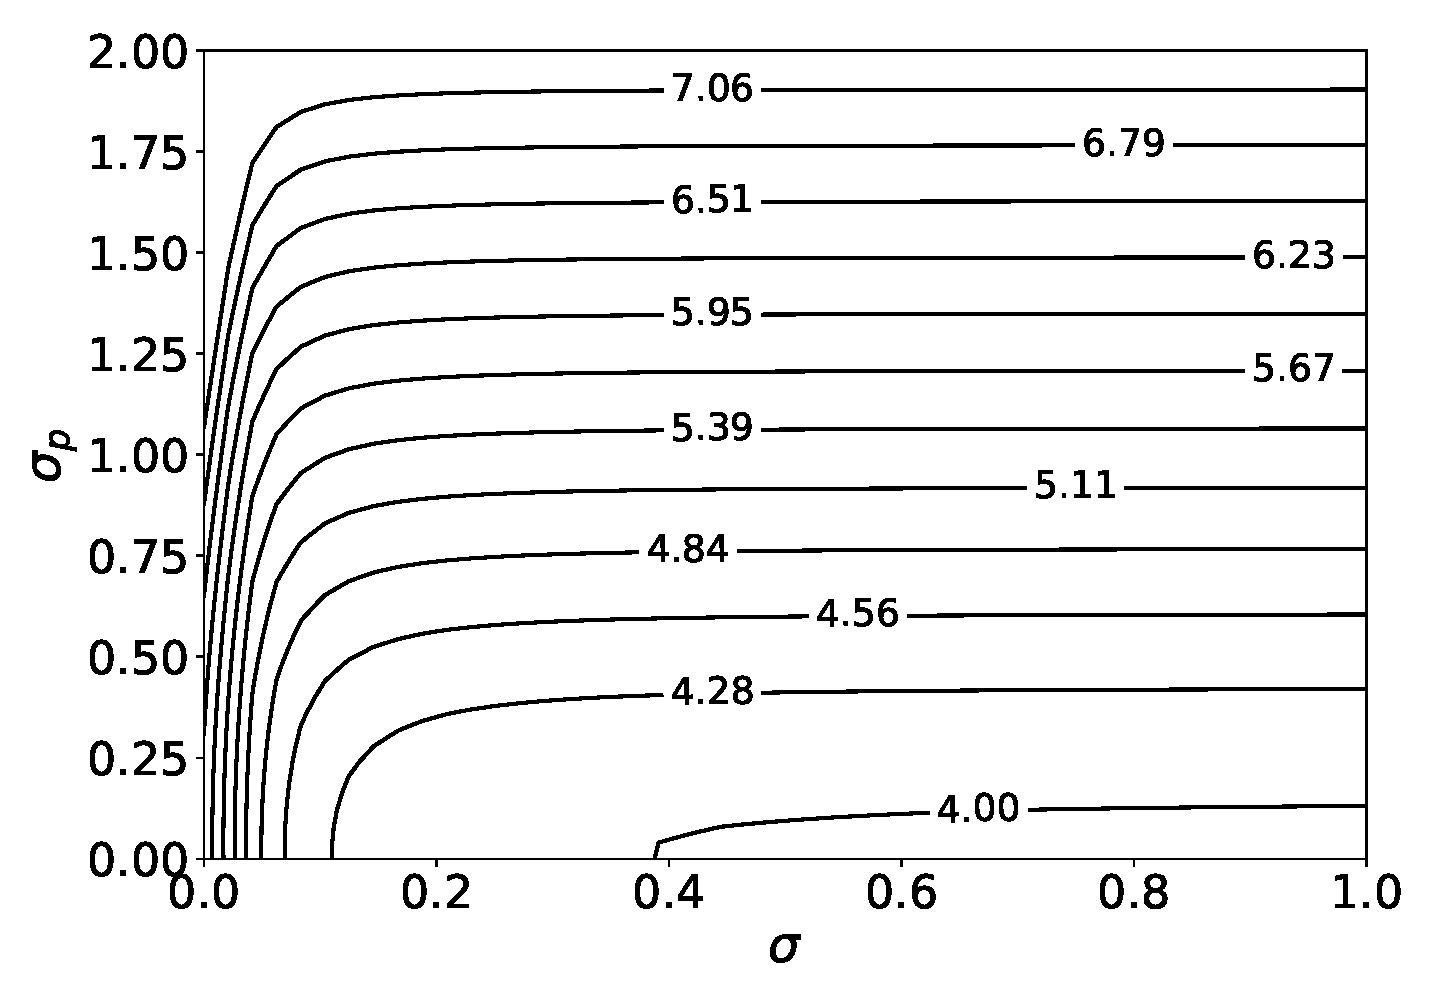
\includegraphics{./figures/optimal_ctrl.eps}}
%     % \label{fig:iwp-projections}
%     %
%     % \hspace{5pt}
%     \hfill
%     %
%     \subfloat[The minimal expected cost $\mathbb{E}\mc{J}$.]
%     {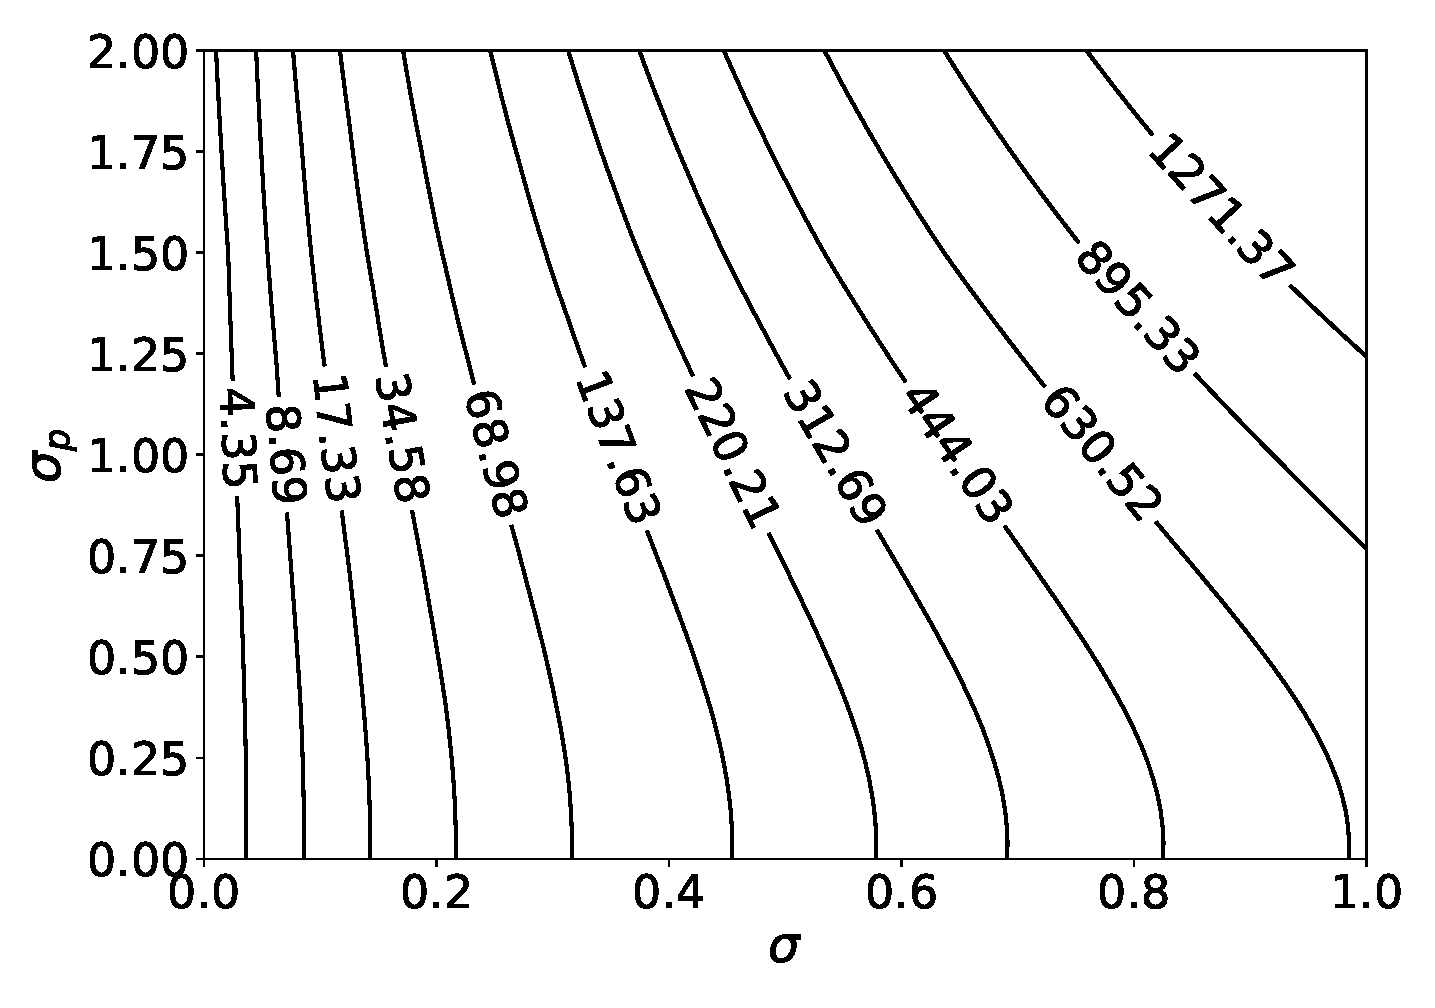
\includegraphics{./figures/optimal_cost.eps}}
%     % \label{fig:iwp-loss}
%     %
%     \caption{As a function of the standard deviations of the measurement noise,
%     $\sigma$, and the system parameter, $\sigma_p$ (a) the magnitude of the optimal
%     controller parameter $\abs{\theta^\star}$ and (b) the minimal expected cost 
%     $\mathbb{E}\mc{J}$.}
%     %
%     \label{fig:optimal-ctrl-cost}
% \end{figure}
